\documentclass{beamer}
\usetheme{metropolis}           % Use metropolis theme

\setbeamercolor{title}{fg=white}
\setbeamercolor{author}{fg=black}
\setbeamercolor{institute}{fg=white}

\newcommand{\todo}{\alert{TODO}}

\title{Mastering the game of Go \\ with deep neural networks and tree search}
\date{}                         % no dates
\author{Karel Ha \\ article by Google DeepMind}
%\author{Google DeepMind \\ presented by Karel Ha}
\institute{Spring School of Combinatorics 2016}

\begin{document}
  {
    \usebackgroundtemplate{
      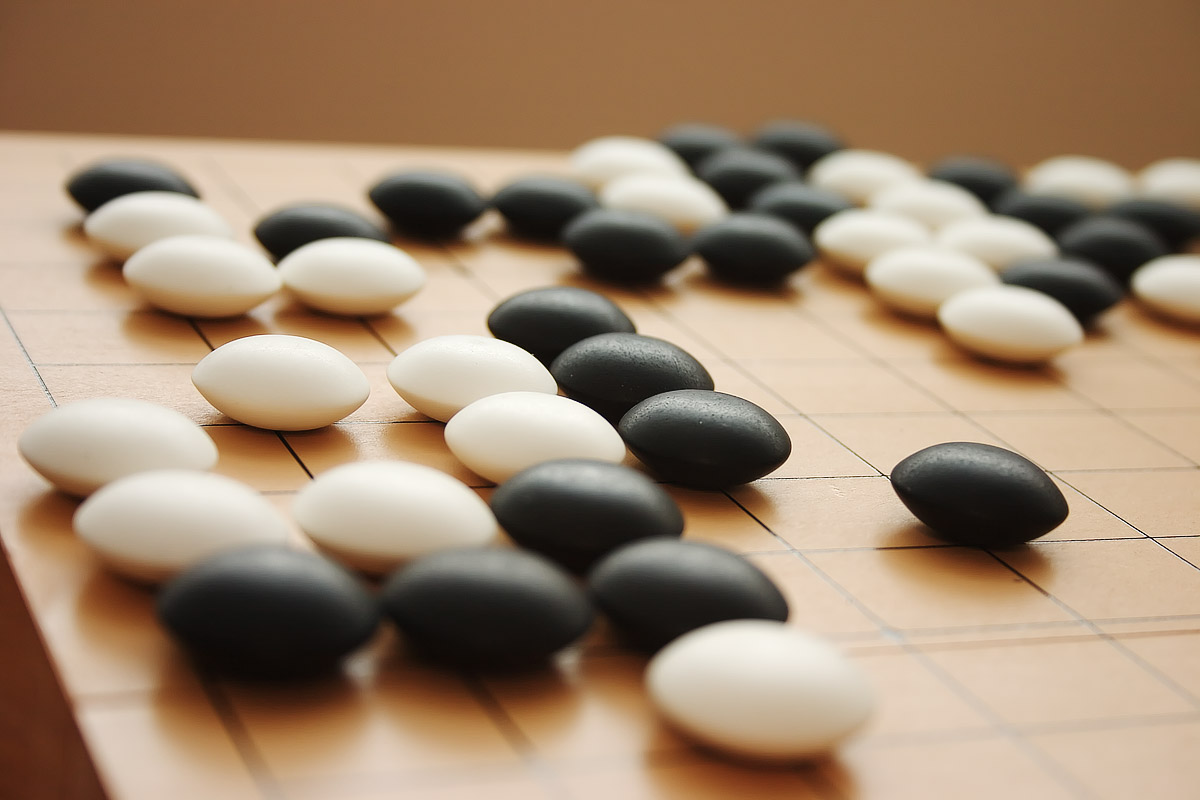
\includegraphics[height=\paperheight]{../img/Go_background.jpg}
    }
    \maketitle
  }

%%%%%%%%%%%%%%%%%%%%%%%%%%%%%%%%%%%%%%%%%%%%%%%%%%%%%%%%%%%%%%%%%%%%%%%%%%%%%%%%

  \section{Why AI?}

  \begin{frame}{Applications of AI}
    \todo
  \end{frame}

  \begin{frame}{Artistic-style painting}
    \begin{center}
      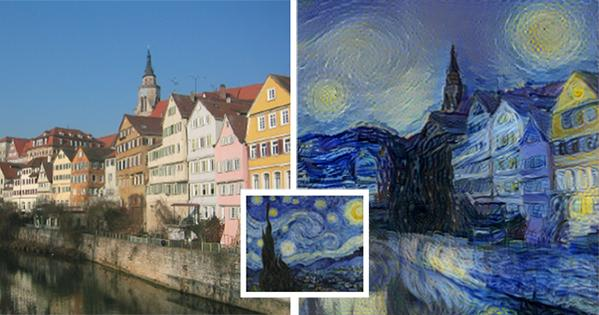
\includegraphics[height=.4\textheight]{../img/art_Van_Gogh.jpg}

      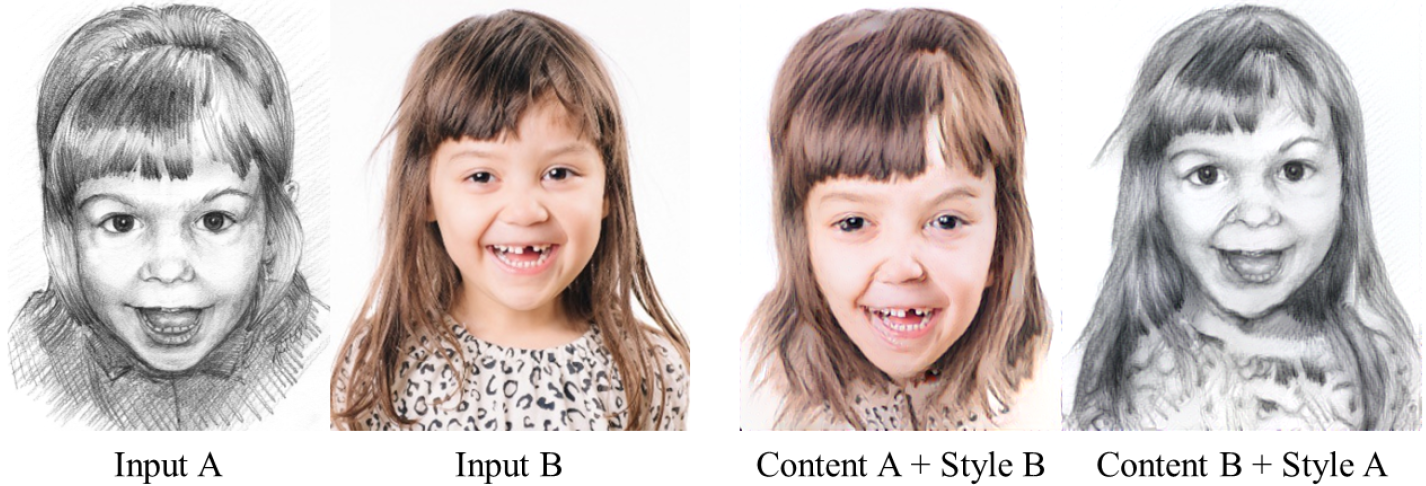
\includegraphics[height=.4\textheight]{../img/art_girl.png}
    \end{center}
  \end{frame}

  \begin{frame}{DeepDrumpf}
    a~Twitter bot that has learned the~language of~Donald Trump from his speeches
    (Bradley Hayes, MIT)
    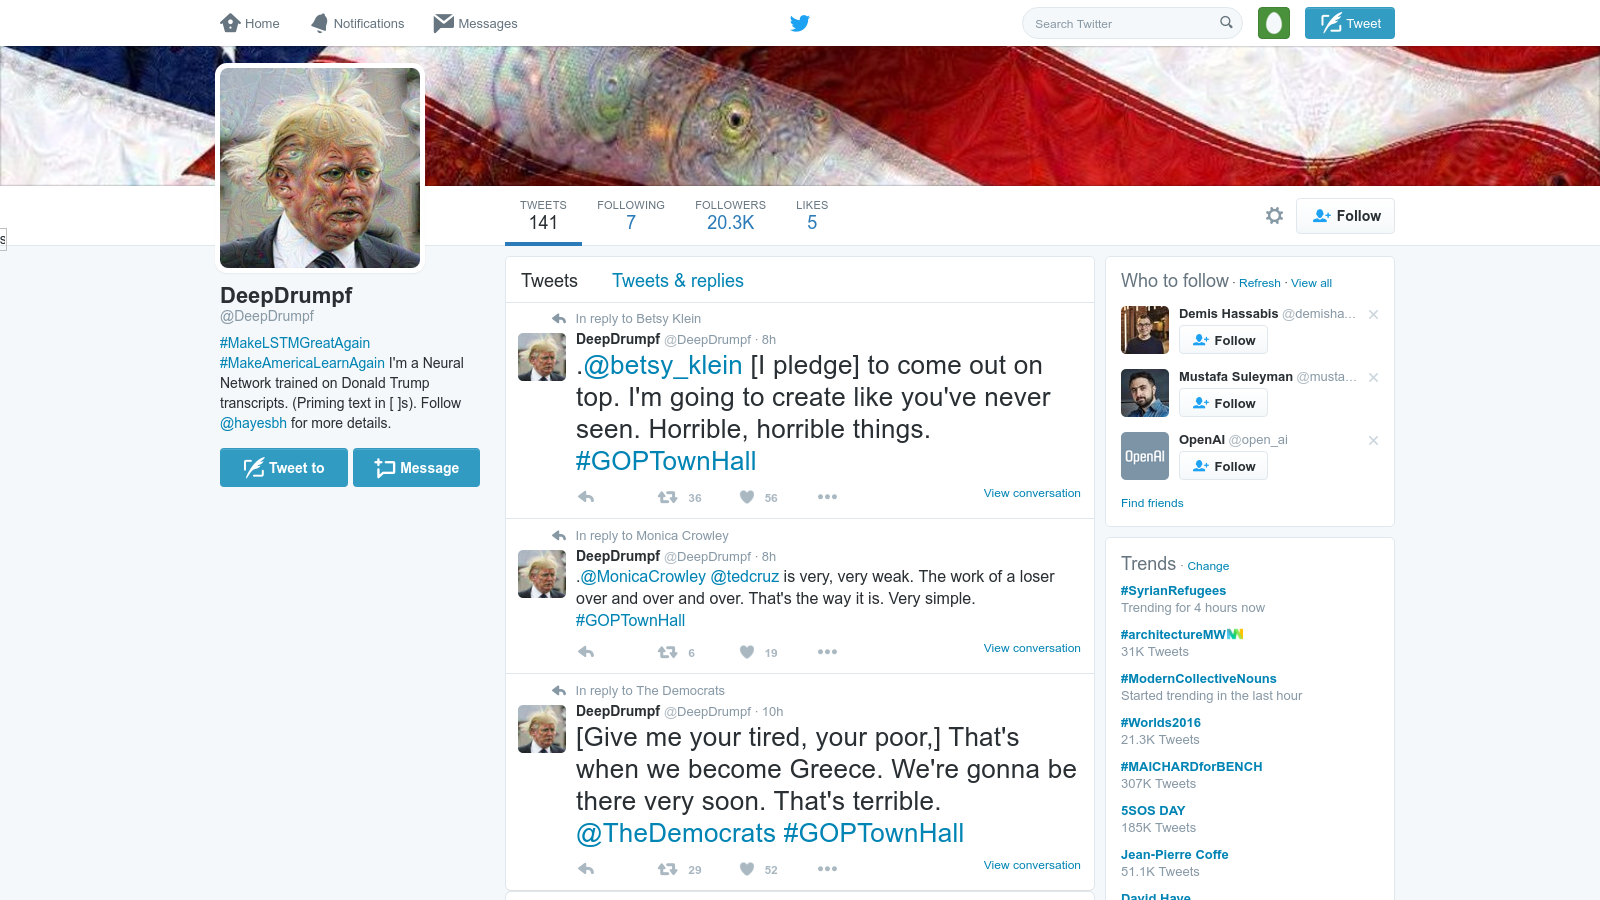
\includegraphics[width=\textwidth]{../img/DeepDrumpf.png}

    \url{https://twitter.com/deepdrumpf}
  \end{frame}

%%%%%%%%%%%%%%%%%%%%%%%%%%%%%%%%%%%%%%%%%%%%%%%%%%%%%%%%%%%%%%%%%%%%%%%%%%%%%%%%

  \section{Basics of Machine learning}
  \begin{frame}{Supervised learning}
    Phases:
    \begin{enumerate}
        % TODO alert only current bullet
        \pause
      \item \alert{collecting data} \todo
        \pause
      \item \alert{training} \todo
        \pause
      \item \alert{testing} \todo
        \pause
      \item \alert{deploying into production} \todo
    \end{enumerate}
  \end{frame}

  \begin{frame}{Unsupervised learning}
    \todo
  \end{frame}

  \begin{frame}{Reinforcement learning}
    \alert{Self-play}
    \todo
  \end{frame}

%%%%%%%%%%%%%%%%%%%%%%%%%%%%%%%%%%%%%%%%%%%%%%%%%%%%%%%%%%%%%%%%%%%%%%%%%%%%%%%%

  \section{Monte Carlo Tree Search}
  \begin{frame}{Game-tree of Go}
    \todo
  \end{frame}

%%%%%%%%%%%%%%%%%%%%%%%%%%%%%%%%%%%%%%%%%%%%%%%%%%%%%%%%%%%%%%%%%%%%%%%%%%%%%%%%

  \section{Neural networks}
  \begin{frame}{Neural network}
    \todo
  \end{frame}

  \begin{frame}{Deep neural network}
    \todo
  \end{frame}

  \begin{frame}{Convolutional neural network}
    \todo
  \end{frame}

%%%%%%%%%%%%%%%%%%%%%%%%%%%%%%%%%%%%%%%%%%%%%%%%%%%%%%%%%%%%%%%%%%%%%%%%%%%%%%%%

  \section{Rules of Go}
  \begin{frame}{Rules of Go}
    \emph{Black} versus \emph{White}.
    Black starts the game.

    \pause
    Two rules:
    \begin{description}
      \item [the rule of liberty] \todo
      \item [the ``ko'' rule] \todo
    \end{description}

    \pause
    \emph{Handicap} for difference in rank:
    Black can place 2 or more stones in advance (compensation for White's greater strength).
  \end{frame}

  \begin{frame}{Ranks}
    \todo
  \end{frame}

%%%%%%%%%%%%%%%%%%%%%%%%%%%%%%%%%%%%%%%%%%%%%%%%%%%%%%%%%%%%%%%%%%%%%%%%%%%%%%%%

  \section{AlphaGo: Inside Out}
  \begin{frame}{Overview}
    \todo
  \end{frame}

  \subsection{Policy networks}
  \begin{frame}{Rollout policy}
    \todo
  \end{frame}

  \begin{frame}{SL policy networks}
    \todo
  \end{frame}

  \begin{frame}{RL policy networks}
    \todo
  \end{frame}

  \subsection{Value network}
  \begin{frame}{Value network}
    \todo
  \end{frame}

  \subsection{MCTS with neural networks}
  \begin{frame}{MCTS with neural networks}
    \todo
  \end{frame}

  \subsection{Scalability}
  \begin{frame}{Scalability}
    \todo
  \end{frame}

%%%%%%%%%%%%%%%%%%%%%%%%%%%%%%%%%%%%%%%%%%%%%%%%%%%%%%%%%%%%%%%%%%%%%%%%%%%%%%%%

  \section{Results: the strength of AlphaGo}

  \begin{frame}{Tournament with other Go programs}
    \todo
  \end{frame}

  \begin{frame}{AlphaGo vs. Fan Hui}
    \todo
  \end{frame}

  \begin{frame}{AlphaGo vs. Lee Sedol}
    \todo
  \end{frame}

%%%%%%%%%%%%%%%%%%%%%%%%%%%%%%%%%%%%%%%%%%%%%%%%%%%%%%%%%%%%%%%%%%%%%%%%%%%%%%%%

  \section{Conclusion}

  \begin{frame}{Discussion}
    \todo
  \end{frame}

  \begin{frame}
    \begin{center}
      Thank you! \\
      Questions?
    \end{center}
  \end{frame}

\end{document}
